\documentclass{beamer}
\usepackage{amssymb,amsmath,mathrsfs}

\usepackage{epsfig,psfrag,epstopdf}

\newcommand{\sQ}{\mathcal{Q}}
\newcommand{\nc}{\mathit{nc}}
\DeclareMathOperator*{\argmin}{arg\,min}

%\usetheme{PaloAlto}
\usetheme{Szeged}
%\usecolortheme{beaver}

\usepackage{graphicx}
\graphicspath{{./figures/}}
\DeclareGraphicsExtensions{.pdf,.eps}

\usepackage{prelim_def}

\newtheorem{massump}{Modeling Assumptions}

\title[Energy Shaping]{A Lyapunov Approach to Orbital \\Stabilization through Energy Shaping}
\subtitle{Applications to Bipedal Walking\\--- Preliminary Results ---}
\author{R. W. Sinnet}
\institute{Department of Mechanical Engineering\\ Texas A\&M University}
\date{July ?, 2014}


\begin{document}

\frame{\titlepage}

\begin{frame}
  \frametitle{Table of Contents}
  \tableofcontents
\end{frame}

\section{Introduction}
\begin{frame}
  \frametitle{intro}
  intro
\end{frame}

\begin{frame}
  \frametitle{Goal}
  goal
\end{frame}

\begin{frame}
  \frametitle{History}
  \begin{columns}[T]

    \begin{column}{.24\textwidth}
      \textcolor{blue}{Passive Walking:}
      \begin{figure}
        \centering
        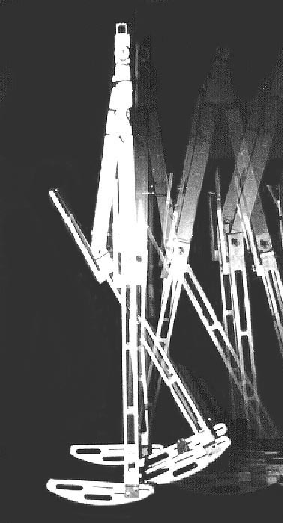
\includegraphics[height=4.5cm]{bipeds_ruina}
      \end{figure}
    \end{column}

    \begin{column}{.24\textwidth}
      \textcolor{blue}{Passivity-Based Control:}
      \begin{figure}
        \centering
        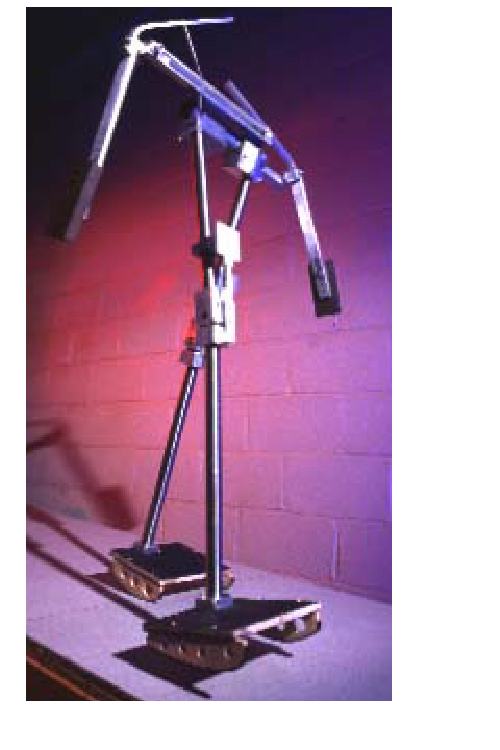
\includegraphics[height=4.5cm]{bipeds_collins}
      \end{figure}
    \end{column}

    \begin{column}{.24\textwidth}
      \textcolor{blue}{Hybrid Zero Dynamics:}
      \begin{figure}
        \centering
        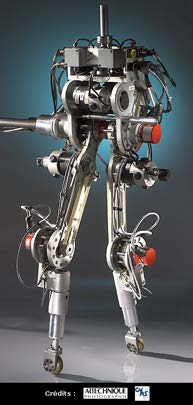
\includegraphics[height=4.5cm]{figures/bipeds_grizzle}
      \end{figure}
    \end{column}

    \begin{column}{.24\textwidth}
      \textcolor{blue}{Human-Inspired Control:}
      \begin{figure}
        \centering
        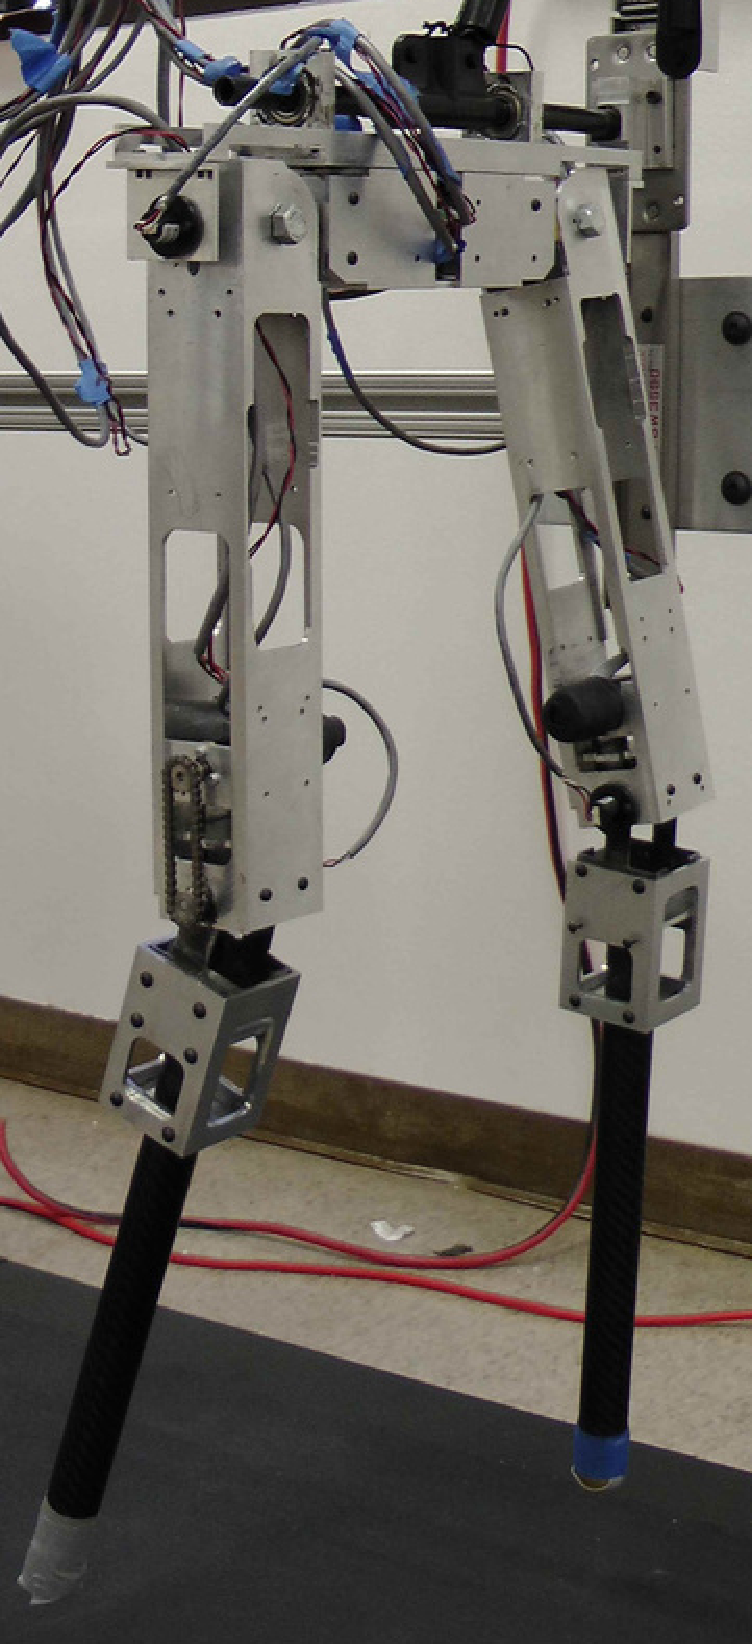
\includegraphics[height=4.5cm]{figures/bipeds_ames}
      \end{figure}
    \end{column}

  \end{columns}
\end{frame}

\section{Mechanics of Bipeds}
\begin{frame}
  \frametitle{Overview}
  \tableofcontents[sectionstyle=show/shaded,subsectionstyle=hide]
\end{frame}

\begin{frame}
  \frametitle{Bipedal Models}
  \begin{figure}
    \centering
    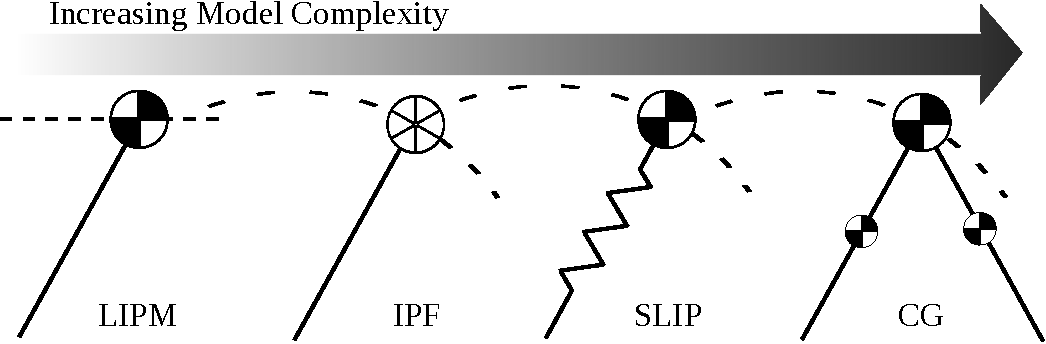
\includegraphics[width=.9\textwidth]{biped-models}
  \end{figure}
  \begin{itemize}
    \item Bipedal locomotion has been studied with a variety of models.
    \item Pendulum models consider massless legs with no impacts.
    \item Kinematic chains are markedly more complex than pendula.
  \end{itemize}
\end{frame}

\begin{frame}
  \frametitle{Hybrid Systems}
  \begin{columns}[t]
    \begin{column}{.63\textwidth}
      \begin{definition}
        A \alert{hybrid control system} is a tuple \vspace{-.3cm}
        $$\HCS = \hcsystem, \vspace{-.4cm}$$
        where
        \begin{itemize}
        \item
          $\Domain \subset \mathcal{X}$ is the {\em domain of admissiblity} with state space $\mathcal{X}$,
        \item
          $\ControlSet$ is a set of {\em admissible controls},
        \item
          $\Guard$ is a {\em guard} or {\em switching surface},
        \item
          $\ResetMap$ is a smooth {\em reset map},
        \item
          $(f, g)$ is a control system on $\Domain$: \vspace{-3mm}
          \begin{align*}
            \dot{x} = f(x) + g(x) \, u.
        \end{align*}
        \end{itemize}
      \end{definition}
    \end{column}
    \begin{column}{.4\textwidth}
      \begin{figure}
        \centering
        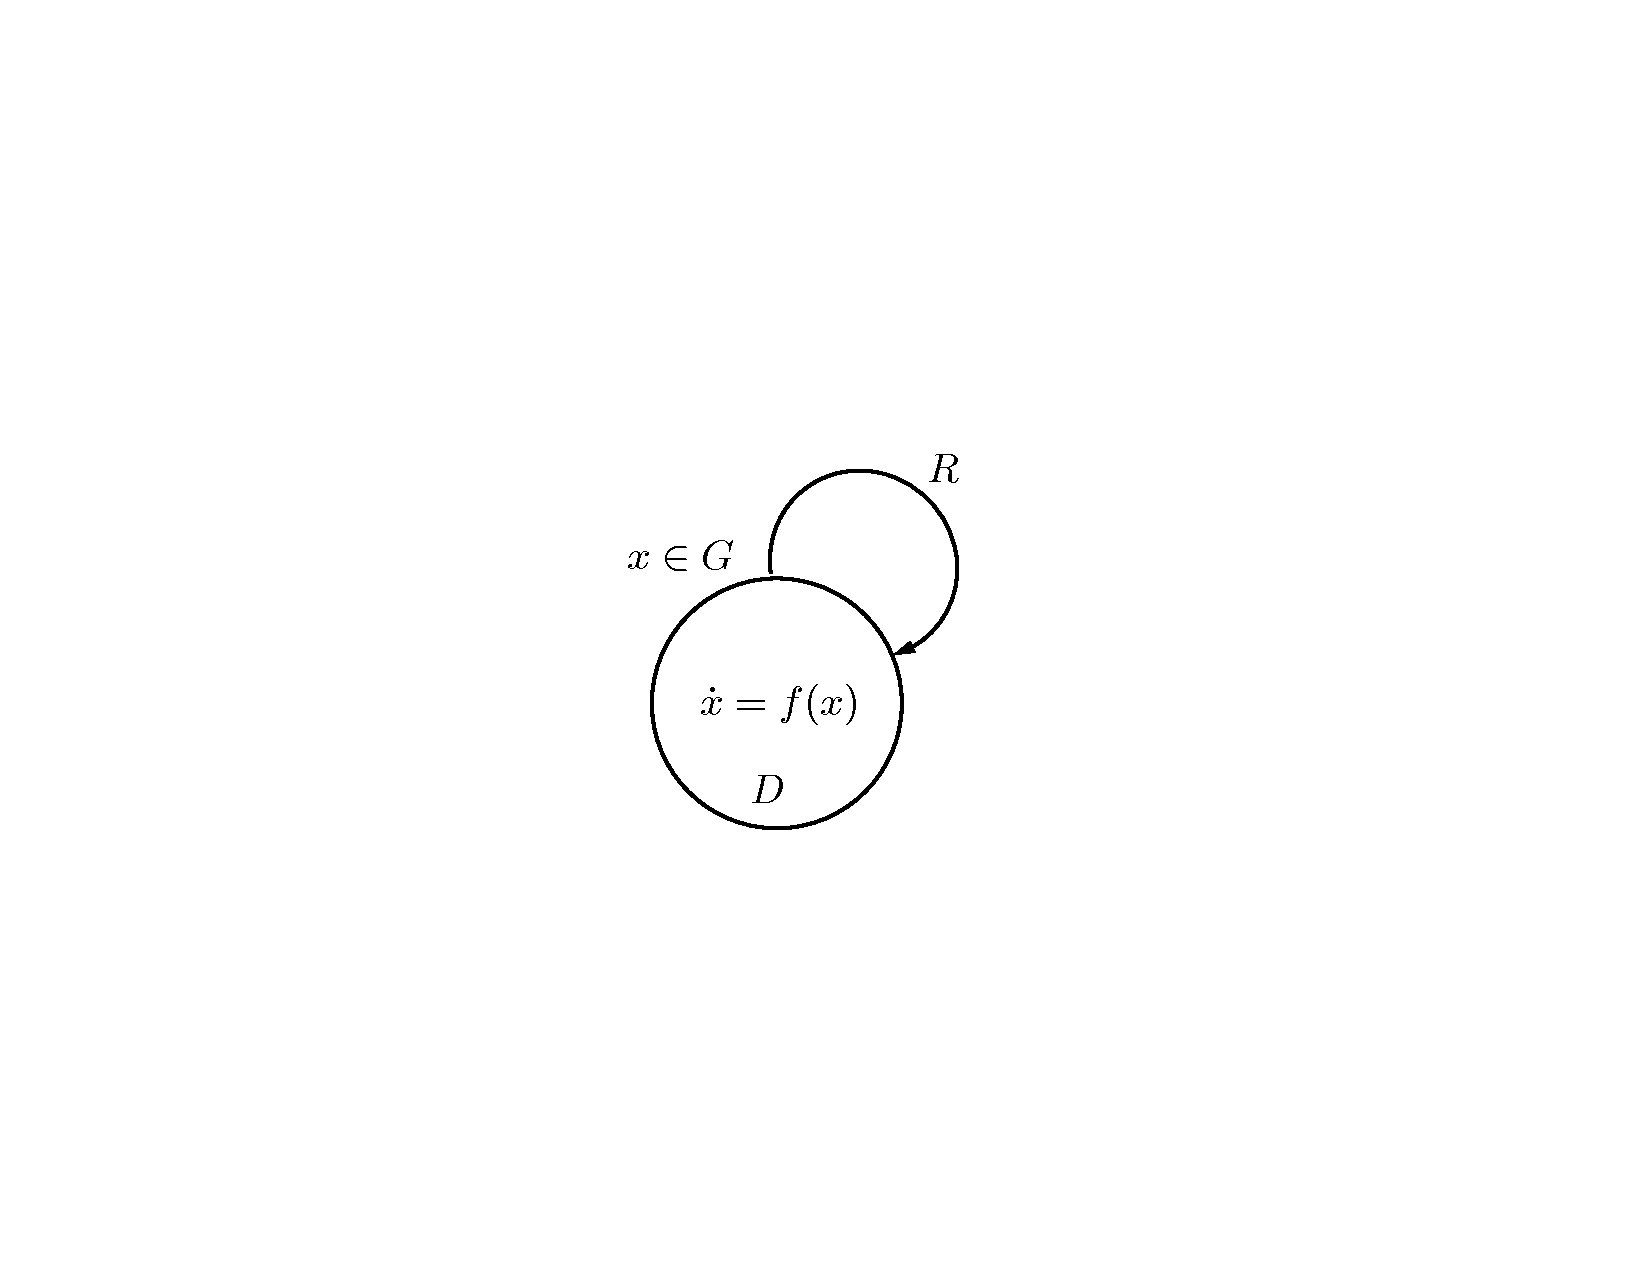
\includegraphics[width=.9\textwidth]{hsystem}\\
      \end{figure}
      A \textcolor{blue}{simple hybrid system}:\vspace{-.3cm}
      $$\HS = \hsystem$$
    \end{column}
  \end{columns}
\end{frame}

\begin{frame}
  \frametitle{Lagrangian Systems}
  Mechanical systems are defined by:
  \begin{itemize}
  \item Kinetic energy, $T : T\sQ \to \R^+$,\\
  \item  Potential energy, $U : \sQ \to \R$,
  \end{itemize}
  which together comprise the total energy,
  \begin{align*}
    E(q, \dot q) = T(q, \dot q) + U(q).
  \end{align*}
  In a Hamiltonian system, energy is conserved and thus the dynamics reflects the flow of energy between $T(q, \dot q)$ and $U(q)$.
\end{frame}

\begin{frame}
  \frametitle{Swing Phase Dynamics}
  \begin{columns}[t]
    \begin{column}{.55\textwidth}
      For Lagrangian $\Lagrangian$ with coordinates
      \begin{align*}
        x = (\q^{T}, \dq^{T})^{T} \in T\ConfigurationSpace,
      \end{align*}
      the principal of least action allows one to construct a dynamic model:
      \begin{align*}
        \D(\q) \, \ddq + \C(\q, \dq) \, \dq + \G(\q) = B(\q) \, u,
      \end{align*}
      or $\dot x = f(q, \dot q) + g(q) \, u,$ with
      \begin{align*}
        f(\q, \dq) &= \left(\!\!\begin{array}{c}
        \dq\\
        \D^{-1}(\q) (-\C(\q, \dq) \, \dq - \G(\q))
        \end{array}\!\!\right),\\
        g(\q) &= \left(\!\!\begin{array}{c}
        \mathbf{0}_{m \times m}\\
        \D^{-1}(\q) B(\q)
        \end{array}\!\!\right).
      \end{align*}
    \end{column}\!\!
    \begin{column}{.45\textwidth}
      \begin{figure}
        \centering
        \vspace{-10mm}
        \caption{Physical configuration}
        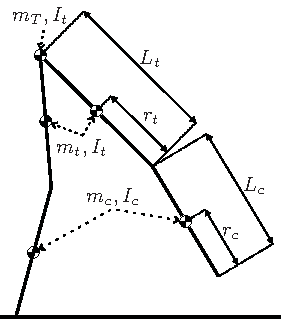
\includegraphics[width = 1.0\columnwidth]{robot_config}
      \end{figure}
    \end{column}
  \end{columns}
\end{frame}

\begin{frame}
  \frametitle{Impact Dynamics}
  Introduce extended coordinates $\qe = (p_{x}, p_{y}, p_{z}, \q^{T})^{T} \in \R^{3} \times \ConfigurationSpace$. Angular momentum balance based on H{\"u}rm{\"u}zl{\"u} and Marghitu:
  \begin{massump}
    \begin{itemize}
    \item Rigid-body plastic impacts
    \item Enough friction to prevent slipping
    \item Impact points do not rebound
    \item Motors do not produce impulses
    \item No instantaneous change in configuration, i.e., $\qe^{-} = \qe^{+}$
    \end{itemize}
  \end{massump}
  Under these assumptions, the discrete dynamics satisfies
  \begin{align*}
    \left[\begin{array}{c c}
        \D_{e}(\qe) & -\Jacobian^{T}(\qe)\\
        \Jacobian(\qe) & \mathbf{0}_{3 \times 3}
      \end{array}\right]
    \left[\begin{array}{c}
        \dq^{+}\\
        \delta F(\qe, \dqe)
      \end{array}\right]
    = \left[\begin{array}{c c}
        \D_{e}(\qe) \, \dqe^{-}\\
        \mathbf{0}_{3}
      \end{array}\right].
  \end{align*}
\end{frame}

\begin{frame}
  \frametitle{Solutions to Dynamical Systems}
  dsys
\end{frame}

\begin{frame}
  \frametitle{Periodic Orbits}
\end{frame}

\begin{frame}
  \frametitle{Conservative Systems}
  csys
\end{frame}


\begin{frame}
  \frametitle{The Simplest Example: Passive Compass-Gait Biped}
  \only<1>{
    \begin{columns}[l]
      \column{1.5in}
      Dynamic Model:
      \begin{align*}
        M(q) \ddot q + H(q, \dot q) = 0
      \end{align*}
      \column{1.5in}
      \begin{figure}
        \centering
        \def\svgwidth{1.0\columnwidth}
        \input{figures/cg2d-slope-model.eps_latex}
        \vspace{-2em}
        \caption{Compass-gait biped falling down a slope.}
      \end{figure}
    \end{columns}
  }
  \only<2>{
    \begin{figure}
      \centering
      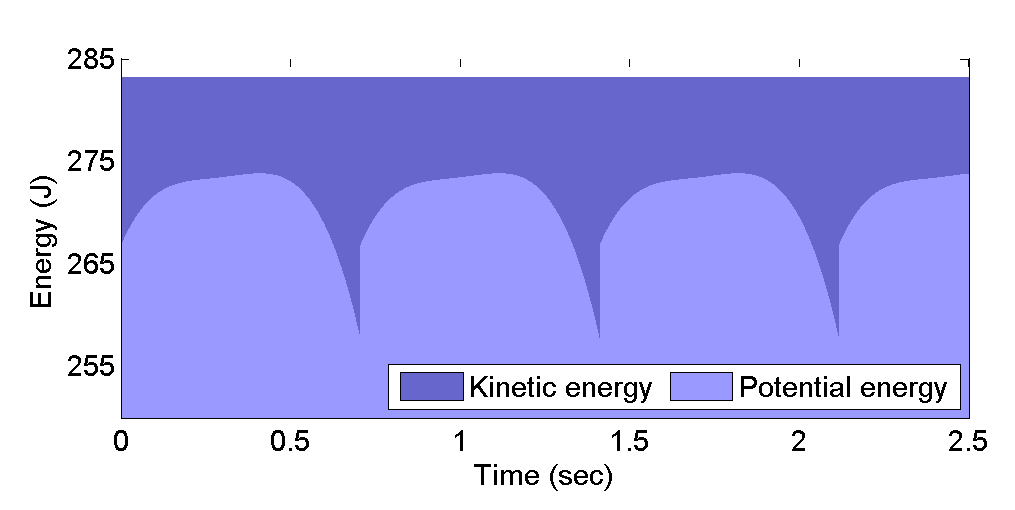
\includegraphics[width=1.0\columnwidth]{energy_cg2d_slope_model}
      \caption{Energy is exchanged between kinetic and potential in form.}
    \end{figure}    
  }
\end{frame}

\begin{frame}
  \frametitle{Nonconservative Systems}
  For a nonconservative system, energy flows out of the system at a rate of $F_{\nc} \cdot dq$. Thus, the following quantity is conserved:
  \begin{align*}
    E_{c} &= T(q, \dot q) + U(q) - \int_{t_{0}}^{t_{1}} \! F_{\nc} \cdot dq\\
    &= E(q(0), \dot q(0)) = E_{0}
  \end{align*}
  This equation expresses the interplay between kinetic and potential energy and the flow of energy into and out of the system.
\end{frame}

\begin{frame}
  \frametitle{Example: 3-Link Biped}
  \only<1>{
    \begin{columns}[l]
      \column{1.5in}
      Dynamic Model:
      \begin{align*}
        M(q) \ddot q + H(q, \dot q) = 0
      \end{align*}
      Control Law:
      \begin{align*}
        u_1 &=-k_{d} (\dot \vartheta_{T}^{a})\\
        &\hspace{1.8em} -k_{p} (\vartheta_{T}^{a} - \vartheta_{T}^{d}),\\
        u_2 &= G(q) - G(\Psi(q)).
      \end{align*}
      \column{1.5in}
      \begin{figure}
        \centering
        \def\svgwidth{1.0\columnwidth}
        \input{figures/cg2d-3link-model.eps_latex}
        \vspace{-2em}
        \caption{3-link biped configuration.}
      \end{figure}
    \end{columns}
  }

  \only<2>{
    \begin{figure}
      \centering
      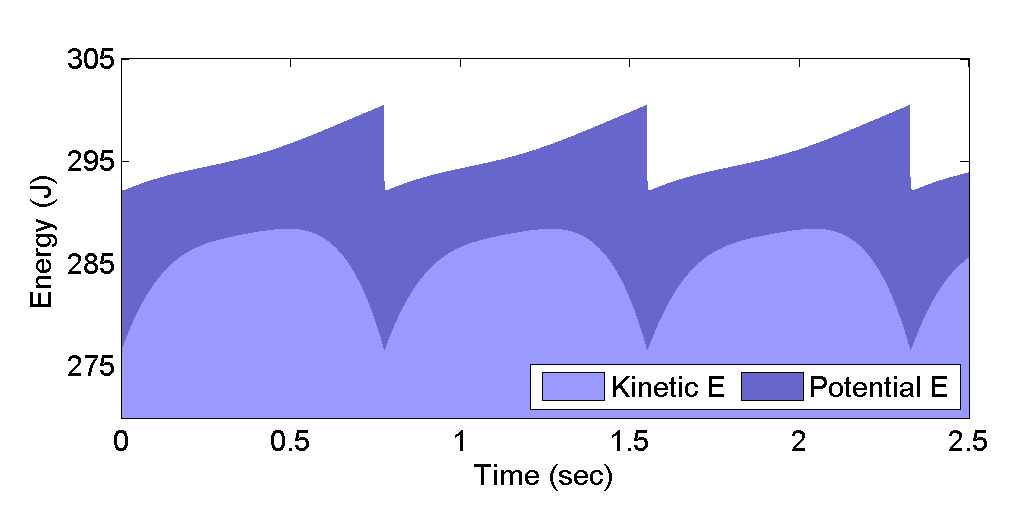
\includegraphics[width=1.0\columnwidth]{energy_cg2d_3link}
      \caption{Energy is not conserved as the controller injects energy.}
    \end{figure}
  }
\end{frame}

\section{Orbital Stabilization}

\begin{frame}
  \frametitle{Orbital Stability}
  \begin{itemize}
  \item Periodic orbits have associated energy levels which define a hypersurface.
  \item We can stabilize to an energy level.
  \end{itemize}
\end{frame}


\begin{frame}
  \frametitle{Energy Shaping}
  Define the output $\eta = E_{c}(q, \dot q) - E_{0}$.
  Control Lyapunov Function
\end{frame}

\begin{frame}
  \frametitle{Quadratic Programming}
  \begin{align}
    \nonumber
    \argmin_{v = (\delta, u)}  \, & v^T \! H \, v + h^T(q, \dot q) v\\
    \label{clf} \tag{clf}
    \mbox{s.t. } & A_{\mathit{clf}}(q, \dot q) v \leq b_{\mathit{clf}}(q, \dot q)\\
    \label{lim} \tag{lim}
    & A_{\mathit{lim}} v \leq b_{\mathit{lim}}
  \end{align}
  where
  \begin{align*}
    H = \left(\begin{array}{c c}\epsilon & 0\\ 0 & I\end{array}\right), \qquad h(q, \dot q) = -2 \, \bar u(q, \dot q)
  \end{align*}
  and
  \begin{itemize}
  \item\eqref{clf} imposes the control Lyapunv function
  \item\eqref{lim} imposes torque limits
  \end{itemize}
  %The above acts to stabilize the energy of the system while attempting to obey the nominal system dynamics.
\end{frame}

\begin{frame}
  \frametitle{Example: Compass Gait}
  compass gait
\end{frame}

\begin{frame}
  \frametitle{Nonconservative Systems}
  nconsys
\end{frame}

\begin{frame}
  \frametitle{Example: 3-Link Biped}
  \only<2>{
    \begin{figure}
      \centering
      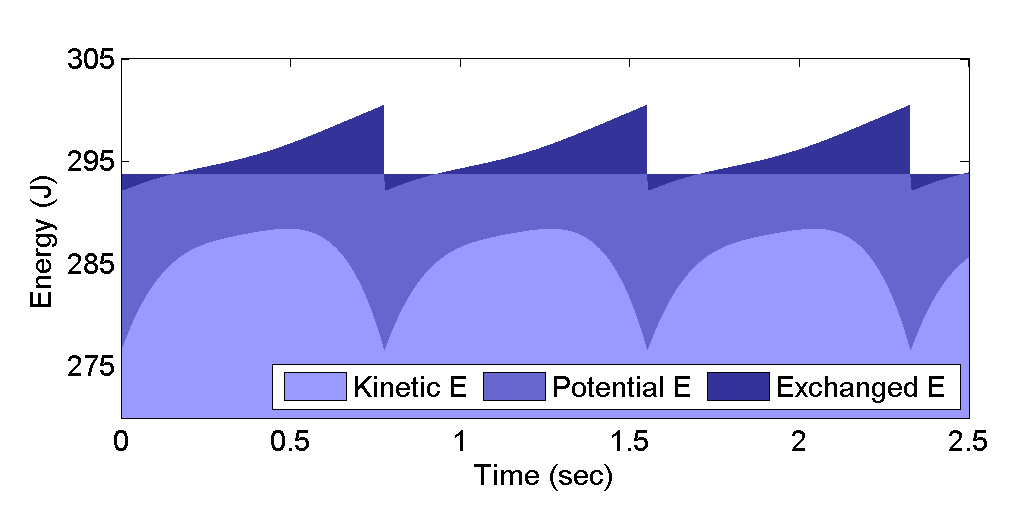
\includegraphics[width=1.0\columnwidth]{energy_conserved_cg2d_3link}
      \caption{The quantity, $E_{0} \equiv T(q, \dot q) + V(q) + \int_{0}^{t} F_{nc} \cdot dq$, is conserved.}
    \end{figure}
  }
\end{frame}

\section{Functional Routhian Reduction}
\begin{frame}
  \frametitle{Overview}
  diagram
\end{frame}

\begin{frame}
  \frametitle{Almost Cyclic Lagrangians}
  ac lags
\end{frame}

\begin{frame}
  \frametitle{Reduction Theorem}
  thm
\end{frame}

\begin{frame}
  \frametitle{Lagrangian Shaping}
  lag shaping
\end{frame}

\begin{frame}
  \frametitle{Reduction Surface Stabilization}
  surf stab
\end{frame}

\section{Results and Remaining Work}
\begin{frame}
  \frametitle{Walking with Feet}
  \begin{itemize}
  \item 2D biped with feet
  \end{itemize}
\end{frame}

%% \section{Conclusions}
%% \begin{frame}
%%   \frametitle{Conclusions}
%%   con.
%% \end{frame}

%\section{Hybrid Systems}
%
%\subsection{Formalisms}
%\frame{hsys}
%
%\section{Hybrid Models}
%\frame{hmodels}
%
%\section{Controlled Lagrangians}
%\begin{frame}
%  \begin{itemize}
%    \item Explain the significance of energy in mechanical systems.
%  \end{itemize}
%\end{frame}

%\section{Energy Shaping}
%\frame{ES}
%\begin{frame}
%  \frametitle{Formulation}
%  s
%\end{frame}


%% \begin{frame}
%%   \frametitle{A Simple Example}
%%   The pendulum can be stabilized to a given level set of the energy.
%% \end{frame}
%% 


\end{document}
